\subsection{REST API Details}

%List here a few resources retrievable via REST API

\subsubsection*{Register Form}

% the description of the resource

REST API details for the Register form include endpoints and request/response formats for handling user registration. The form collects essential user details such as email, first name, last name, birth date, address, phone number, nationality, password, and license number.



\begin{itemize}
    \item URL: \texttt{/createCostumer}
    \item Method: \texttt{Post}
    % \item URL Parameters:
    \item Data Parameters: \\
\begin{figure}[h]
\centering
\includegraphics[width=0.8\textwidth, inner]{sections//BLL//DataParameter1.jpg}
\caption{Register Form Data Parameter}
\label{fig:figure1}
\end{figure}
    \item Success Response:
\begin{figure}[h]
\centering
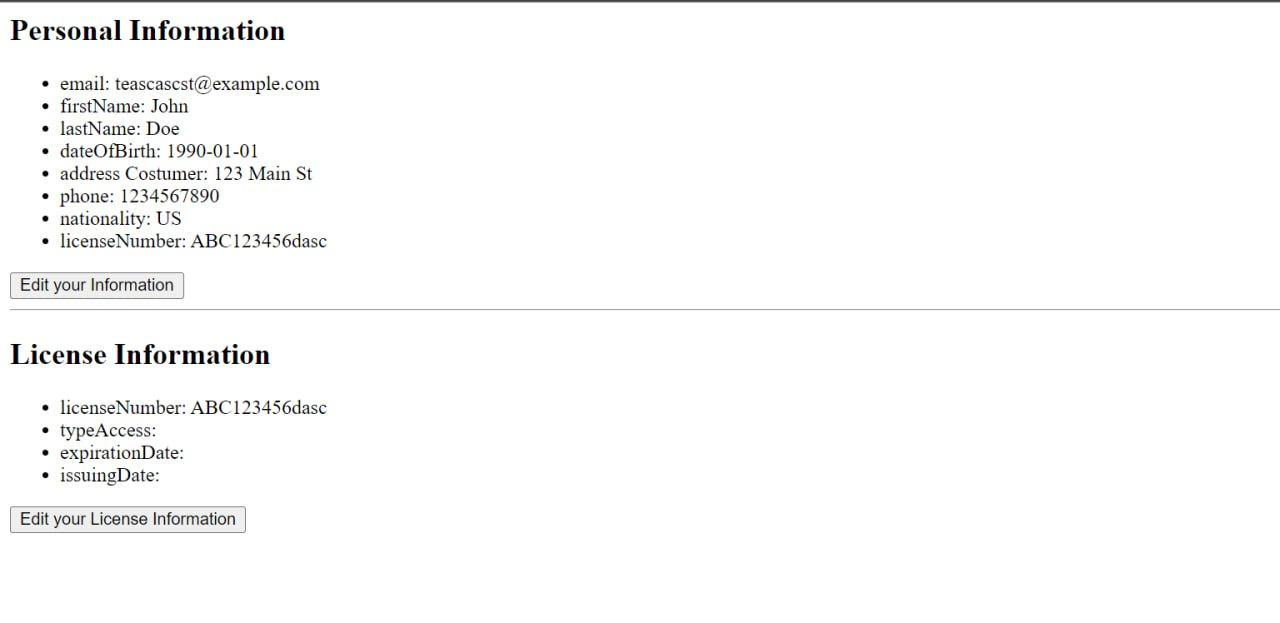
\includegraphics[width=0.8\textwidth, inner]{sections//BLL/SuccssResponse1.jpg}
\caption{Create Costumer Success Response}
\label{fig:figure2}
\end{figure}\newpage
    % \item Error Response:
\subsubsection*{Update Car}
    \item URL: \texttt{/updateCar}
    \item Method: \texttt{Post}
    % \item URL Parameters:
    \item Data Parameters: \\
\begin{figure}[h]
\centering
\includegraphics[width=0.8\textwidth, inner]{sections//BLL/DataParameter1.jpg}
\caption{update Car Data Parameter}
\label{fig:figure1}
\end{figure}
    \item Success Response:
\begin{figure}[h]
\centering
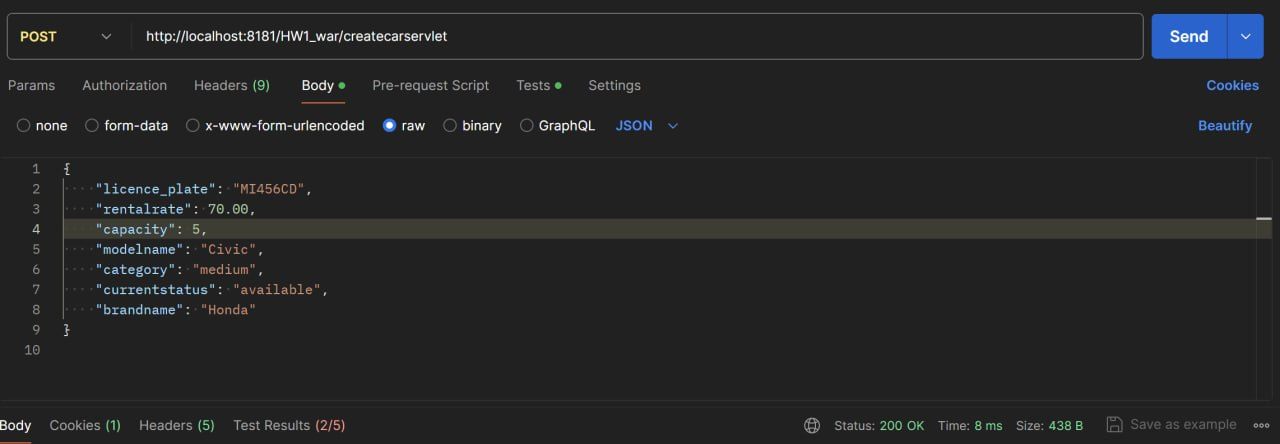
\includegraphics[width=0.7\textwidth, inner]{sections//BLL/updateCar1.jpg}
\caption{Update Car Success Response}
\label{fig:figure1}
\end{figure}\newpage
\newpage
    
\end{itemize}

\subsubsection*{CAR REST APIs}
Here we show some spesific REST API endpoints for managing the car entity. this APIs are under "/rest/car" URL:

\begin{itemize}
    \item URL: \texttt{the URL to retrieve it : /rest/car}
    \item Method: \texttt{Method to retrieve it: GET}
    \item URL Parameters: none
    \item Data Parameters: none
    \item Success Response: 
        \begin{lstlisting}[ style=jsonStyle, caption={ Response Example }, label={lst:json}]
        {
          "resource-list": [
            {
              "car": {
                "licenseplate": "HR23791B",
                "rentalrate": 50.0,
                "capacity": 5,
                "category": "medium",
                "currentstatus": "available",
                "brandname": "Toyota"
              }
            },
            {
              "car": {
                "licenseplate": "T6237FX5",
                "rentalrate": 70.0,
                "capacity": 4,
                "category": "small",
                "currentstatus": "available",
                "brandname": "Honda"
              }
            }
          ]
        }
        \end{lstlisting}
        
    \item Error Response: 
        \begin{lstlisting}[ style=jsonStyle, caption={ Possible Errors }, label={lst:json}]
        500 :  Internal Server Error
    \end{lstlisting}

    
\end{itemize}

\begin{itemize}
    \item URL: \texttt{the URL to retrieve it : /rest/car}
    \item Method: \texttt{Method to retrieve it: POST}
    \item URL Parameters: none
    \item Data Parameters: 
      \begin{lstlisting}[ style=jsonStyle, caption={ Response Example }, label={lst:json}]
        {
            "car":{
            "licenseplate":"H3361WE0",
            "rentalrate": 60.0,
            "capacity": 4,
            "category":"medium",
            "currentstatus":"available",
            "modelname": "X5",
            "brandname": "BMW"
        
            }
        }
        
        \end{lstlisting}
    \item Success Response: 
        \begin{lstlisting}[ style=jsonStyle, caption={ Response Example }, label={lst:json}]
       {
            "car":{
            "licenseplate":"H3361WE0",
            "rentalrate":60.0,
            "capacity":4,
            "category":"medium",
            "currentstatus":"available",
            "brandname":"BMW"
            }
        }
        \end{lstlisting}
    \item Error Response: 
        \begin{lstlisting}[ style=jsonStyle, caption={ Possible Errors }, label={lst:json}]
        500 :  Internal Server Error (Cannot create the car: unexpected error. | Cannot create the car: unexpected database error.)
        400 : Bad Request (Cannot create the car: no Car JSON object found in the request.)
        409: Conflict (Cannot create the car: it already exists.)
        \end{lstlisting}
\newpage
    
\end{itemize}

\begin{itemize}
    \item URL: \texttt{the URL to retrieve it : /rest/car/\{licenceplate\}}
    \item Method: \texttt{Method to retrieve it: GET}
    \item URL Parameters: none
    \item Data Parameters:none
    \item Success Response: 
        \begin{lstlisting}[ style=jsonStyle, caption={ Response Example }, label={lst:json}]
       {
            "car":{
            "licenseplate":"H3361WE0",
            "rentalrate":60.0,
            "capacity":4,
            "category":"medium",
            "currentstatus":"available",
            "brandname":"BMW"
            }
        }
        \end{lstlisting}
    \item Error Response: 
        \begin{lstlisting}[ style=jsonStyle, caption={ Possible Errors }, label={lst:json}]
        500 :  Internal Server Error (Cannot get car: unexpected error. | Cannot get car(s): unexpected database error.)
        \end{lstlisting}
\newpage
    
\end{itemize}

\newpage
    
\end{itemize}

\begin{itemize}
    \item URL: \texttt{the URL to retrieve it : /rest/car/\{licenceplate\}}
    \item Method: \texttt{Method to retrieve it: DELETE}
    \item URL Parameters: none
    \item Data Parameters:none
    \item Success Response: 
        \begin{lstlisting}[ style=jsonStyle, caption={ Response Example }, label={lst:json}]
       {
            "car":{
            "licenseplate":"H3361WE0",
            "rentalrate":60.0,
            "capacity":4,
            "category":"medium",
            "currentstatus":"available",
            "brandname":"BMW"
            }
        }
        \end{lstlisting}
    \item Error Response: 
        \begin{lstlisting}[ style=jsonStyle, caption={ Possible Errors }, label={lst:json}]
        500 :  Internal Server Error (Cannot delete the car: unexpected database error.)
        404 : Not Found ("Car " + lisenceplate + " not found. Cannot delete it." | Cannot delete the car: wrong format for URI /car/{licenceplate}.)
        409: Conflict (Cannot delete the car: other resources depend on it.)
        
        \end{lstlisting}
\newpage
    
\end{itemize}
